%!TEX program = xelatex
\documentclass[12pt]{article}

% ---------- IDIOMA ----------
% --- Paquetes para XeLaTeX y codificación moderna ---
\usepackage{fontspec} 
\usepackage[spanish, es-tabla]{babel} 
% --- Cambiar "Cuadro" por "Tabla" ---
\addto\captionsspanish{\renewcommand{\tablename}{Tabla}}

% ---------- FUENTES ----------
\setmainfont{TeX Gyre Termes}

% ---------- PAQUETES MATEMÁTICOS Y FÍSICOS ----------
\usepackage{amsmath,amssymb}
\usepackage{amsfonts}
\usepackage{physics}

% ---------- GRÁFICOS Y COLORES ----------
\usepackage{xcolor}
\usepackage{graphicx}
\usepackage{tikz}
\usetikzlibrary{babel} % <- Agrega esta línea
\usepackage{tikz-3dplot}
\usetikzlibrary{shapes, arrows, positioning, calc}
\usetikzlibrary{arrows.meta} 
\usetikzlibrary{shapes.geometric} 
\usetikzlibrary{decorations.markings}

% ---------- CÓDIGO (LISTINGS) ----------
\usepackage{listings}

\definecolor{codegreen}{rgb}{0,0.6,0}
\definecolor{codegray}{rgb}{0.95,0.95,0.95}
\definecolor{codepurple}{rgb}{0.58,0,0.82}
\definecolor{backcolour}{rgb}{0.96,0.96,0.96}

\lstdefinestyle{pythonstyle}{
    backgroundcolor=\color{backcolour},   
    commentstyle=\color{codegreen},
    keywordstyle=\color{magenta},
    numberstyle=\tiny\color{gray},
    stringstyle=\color{codepurple},
    basicstyle=\ttfamily\small,          
    breakatwhitespace=false,         
    breaklines=true,                     
    captionpos=b,                    
    keepspaces=true,                 
    numbers=left,                        
    numbersep=5pt,                  
    showspaces=false,                
    showstringspaces=false,
    showtabs=false,                  
    tabsize=4,
    language=Python                      
}
\lstset{style=pythonstyle}

% ---------- DISEÑO Y ESTILO ----------
\usepackage{geometry}
\geometry{letterpaper, margin=2cm, headheight=15pt}
\usepackage{fancyhdr} 
\usepackage{lastpage} 
\usepackage{wrapfig}
\usepackage{multicol}
\usepackage{enumitem}
\usepackage{framed}
\usepackage{etoolbox}

% ---------- TCOLORBOX ----------
\usepackage[most,skins,theorems]{tcolorbox}

% --- Caja para Definiciones Formales ---
\newtcolorbox{definicion}[1][]{
  enhanced,
  breakable, 
  colback=blue!5!white,
  colframe=blue!75!black,
  fonttitle=\bfseries,
  title={Definición: #1},
  arc=2mm,
  boxrule=0.8pt,
  drop shadow=black!10!white
}

% --- Caja para Tareas ---
\newtcolorbox{problemas}[1][]{
  enhanced,
  breakable, 
  colback=violet!6!white,       
  colframe=violet!45!white,     
  coltitle=violet!40!black,     
  fonttitle=\bfseries,
  title={Problemas: #1},
  arc=2.5mm,                    
  boxrule=0.8pt,
  drop shadow=black!8!white     
}

% --- Caja Libre Verde Menta ---
\newtcolorbox{cajaflex}[1][]{
  enhanced,
  colback=teal!5!white,       
  colframe=teal!50!black,     
  coltitle=teal!10!white,     
  fonttitle=\bfseries,
  code={\ifblank{#1}{}{\tcbset{title={#1}}}},
  arc=2.5mm,                  
  boxrule=0.8pt,
  drop shadow=black!8!white   
}

% ---------- TABLAS Y ELEMENTOS EXTRA ----------
\usepackage{booktabs}   
\usepackage{pifont}     
\usepackage{array}      
\usepackage{caption}    

\newcommand{\lapiz}{\ding{46}\ }

% ---------- ENLACES Y PDF ----------
\usepackage{hyperref}

\definecolor{myblue}{RGB}{20, 20, 120}
\definecolor{myred}{RGB}{220, 30, 30}
\definecolor{mygreen}{RGB}{0, 130, 60}

% Personalización de nombres para \autoref
\def\tableautorefname{Tabla}
\def\figureautorefname{Figura}
\def\equationautorefname{Ecuación}
\def\sectionautorefname{Sección}

% ---------- CONFIGURACIÓN DE ENCABEZADOS (ITM) ----------
\newcommand{\logo}{
\includegraphics[height=3cm]{escudoitm}}
\newcommand{\escola}{Facultad de Ciencias Exactas y Aplicadas}
\newcommand{\disc}{Física Computacional 1}
\newcommand{\auth}{Robinson Longas Bedoya}
\newcommand{\emaill}{\url{robinsonlongas@itm.edu.co}}
\newcommand{\email}{\url{robinsonlongas3586@correo.itm.edu.co}}
\newcommand{\cabec}{Física Computacional 1}

\hypersetup{
    colorlinks=true,
    linkcolor=blue,
    urlcolor=blue,
    citecolor=blue,
    pdftitle={\cabec\ -- \auth},
    pdfauthor={\auth}
}

% Configuración de estilos de página
\pagestyle{fancy}
\fancyhf{} 

\fancypagestyle{firstpage}{
    \fancyhead[L]{\logo}
    \fancyhead[R]{
        \textsf{\escola \\} 
        \textsf{\disc \\}
        \textsf{\auth \\}
        \textsf{\email \\} 
        \textsf{\emaill}     
    }
    \fancyfoot[R]{\scriptsize Página \thepage~de \pageref{LastPage}}
    \renewcommand{\headrulewidth}{0pt} 
    \renewcommand{\footrulewidth}{0.4pt} 
}

\fancyhead[L]{\textsf{\scriptsize \cabec\ -- \auth\ -- \email\ -- \emaill}}
\fancyfoot[R]{\scriptsize Página \thepage~de \pageref{LastPage}}
\renewcommand{\headrulewidth}{0.4pt} 
\renewcommand{\footrulewidth}{0.4pt} 

\setlength{\parskip}{0.3em}

\begin{document}
		\thispagestyle{firstpage}
		\vspace*{1.5cm}
	
	\begin{center}
		\rule{\textwidth}{0.4pt}
	\end{center}
	
	\begin{itemize}[leftmargin=*,label=\textcolor{red}{\ensuremath{\blacktriangleright}}]
		\item \textbf{Listas}
		\item \textbf{Arreglos de \texttt{numpy}}
		\item \textbf{Matplotlib}
	\end{itemize}
	
	\noindent
	\textbf{\underline{Bibliografía}}
	\begin{itemize}[leftmargin=*, label={\textcolor{blue}{$\bullet$}}]
		\item \textit{Computational Physics, cap. 2}, Mark Newman.
		\item \textit{Programming for computations - Python. Sec. 1.6 y sec. 2.3}, Svein Lingen, Hans Petter Langtangen.
        \item \textit{Introducción a la programación con Python. Capítulo 5.}, Andrés Marzal, Isabel Gracia y Pedro García.
	\end{itemize}
     
    
    Hasta el momento, hemos trabajado con variables simples, como enteros, flotantes y cadenas de texto. Sin embargo, en física es común
    trabajar con colecciones de datos. Pro ejemplo, un vector en 3 dimensiones tiene asociadas tres componentes $x, y, z$. Una matriz de 3x3 
    tiene asociadas nueve componentes. En general, podemos tener una colección de datos que queremos almacenar y manipular.
    En Python, podemos almacenar estos datos en varios tipos de objetos: diccionarios, tuplas, conjuntos, 
    listas y arreglos. Por ahora, vamos a estudiar las listas y los arreglos. Al final del curso, 
    veremos un poco sobre diccionarios.


\section*{\textcolor{red}{\textit{Listas}}}
	Como su nombre lo indica, una \textit{lista} es un objeto que contiene elementos en secuencia. 
    Por lo general usamos siempre elementos numéricos, pero pueden ser de cualquier tipo. 

    Por ejemplo, \lstinline|lista = [3, 8.9, 'verde', 4. + 3j]|, representa una lista en Python. 
%
\begin{lstlisting}[language=Python]
In [1]: x = 10

In [2]: y= 3.5

In [3]: r = [x, y, x**2 + y, y/x]

In [4]: print("la lista es",r)
la lista es [10, 3.5, 103.5, 0.35]

In [6]: r[0]
Out[6]: 10

In [7]: r[-1]
Out[7]: 0.35
\end{lstlisting}    
%
Supongamos por ejemplo que tenemos un vector $\vec v = \langle 2.1, ~3, ~5\rangle$ y queremos
calcular su magnitud:
%
\begin{lstlisting}[language=Python]
In [8]: import math

In [9]: v = [2.1, -3, 5]

In [10]: norma = math.sqrt(v[0]**2 + v[1]**2 + v[2]**2)

In [11]: print(f"La magnitud del vector v es {norma: .3f}")
La magnitud del vector v es  6.198
\end{lstlisting}    
%

La primera línea importa el módulo \lstinline|math| para calcular la raíz cuadrada.
La segunda línea crea la lista que representa el vector $\vec v$ y la tercera línea calcula la raíz
cuadrada de cada componente al cuadrado. Note que Python por convención comienza  a contar desde cero, 
es decir, el primer elemento es \lstinline|v[0]|. Finalmente, la cuarta línea imprime el resultado con tres 
cifras decimales. Algunas propiedades de las listas son:

\begin{description}
 \item[\textbf{\textcolor{blue}{\textit{1. Mutabilidad:}}}] 
A diferencia de las tuplas o de las cadenas de texto, las listas en Python son 
\textbf{mutables}, lo que significa que podemos modificar sus elementos, 
añadir nuevos datos o eliminar partes de la estructura sin necesidad de redefinirla por completo.

\begin{lstlisting}[language=Python]
In [12]: datos = [1.0, 2.5, 3.8]

# Modificar un elemento existente por su indice
In [13]: datos[1] = 9.9
In [14]: print(datos)
[1.0, 9.9, 3.8]

# Anadir un nuevo elemento al final con .append()
In [15]: datos.append(5.2)
In [16]: print(datos)
[1.0, 9.9, 3.8, 5.2]

# Consultar el numero de elementos de la lista
In [17]: len(datos)
Out[17]: 4
\end{lstlisting}
%
La función \lstinline|.append()| ya la hemos usado cuando estudiamos las estructuras de 
control. Recordemos que un truco que usamos fue definir una lista vacía y luego ir llenándola 
con un bucle \lstinline|for|. Recuerde el programa \textit{tiempo$\_$vuelo.py}.

\item[\textbf{\textcolor{blue}{\textit{2. Slicing (Rebanado):}}}] 

De una lista se puede extraer sublistas especificando un rango de índices. La sintaxis es 
\begin{center}
\lstinline|lista[inicio:fin:paso]|\,,    
\end{center}
 donde \texttt{inicio} es incluyente y \texttt{fin} es excluyente:

\begin{lstlisting}[language=Python]
In [18]: L = [10, 20, 30, 40, 50, 60]

# Sublista desde el indice 1 hasta el 3 (excluye el 4)
In [19]: L[1:4]
Out[19]: [20, 30, 40]

# Omitir el inicio equivale a comenzar desde el indice 0
In [20]: L[:3]
Out[20]: [10, 20, 30]

# Invertir la lista con paso negativo
In [21]: L[::-1]
Out[21]: [60, 50, 40, 30, 20, 10]
\end{lstlisting}

\item[\textbf{\textcolor{blue}{\textit{3. Listas por Comprensión:}}}] 

Una forma compacta y elegante de aplicar operaciones a todos los elementos de una lista sin escribir 
bucles \lstinline|for| en varias líneas es mediante las \textit{listas por comprensión}.
Supongamos que queremos de nuevo calcular la magnitud del vector $\vec v = \langle 2.1, ~3, ~5\rangle$

\begin{lstlisting}[language=Python]
In [14]: v = [2.1, -3, 5]

In [15]: v_cuadrado = [i**2 for i in v]

In [16]: v_cuadrado
Out[16]: [4.41, 9, 25]

In [17]: norma = math.sqrt(sum(v_cuadrado))

In [18]: norma
Out[18]: 6.1975801729384665

In [19]: print(f"La magnitud del vector v es {norma: .3f}")
La magnitud del vector v es  6.198
\end{lstlisting}
%

\item[\textbf{\textcolor{blue}{\textit{4. Función map:}}}] 
Una función especial que se utiliza pra trabajar con listas es \lstinline|map|, que nos permite aplicar 
una función a todos los elementos de una lista. Por ejemplo, podemos calcular el logaritmo al vector 
$\vec a  = [ 1, 2.3, 10.]$ 
de la siguiente manera:
\begin{lstlisting}[language=Python]
In [24]: import math

In [25]: a = [1, 2.3, 10.]

In [26]: loga = list(map(math.log,a))

In [27]: loga
Out[27]: [0.0, 0.8329091229351039, 2.302585092994046]

In [28]: loga10 = list(map(math.log10,a))

In [29]: loga10
Out[29]: [0.0, 0.36172783601759284, 1.0]

In [30]: tana = list(map(math.tan,a))

In [31]: tana
Out[31]: [1.5574077246549023, -1.1192136417341325, 0.6483608274590866]
\end{lstlisting}

\end{description}

\noindent
\textbf{Limitación de las listas en física computacional:}\\
Aunque las listas por comprensión simplifican la sintaxis, realizar operaciones matemáticas elemento a elemento 
sigue requiriendo iterar explícitamente en Python. Como veremos a continuación, para trabajar con millones de datos o 
resolver ecuaciones diferenciales eficientemente, es imprescindible dar el paso a los arreglos de \texttt{numpy}.

\section*{\textcolor{red}{\textit{Numerical Python Arrays (numpy)}}}

A diferencia de las listas que acabamos de ver, los arreglos tienen un número 
de elementos fijo: una vez definidos, no puedes añadir ni quitar elementos. 
Además, deben ser todos del mismo tipo, o enteros o flotantes y una vez creado no 
puedes cambiarlos.

En las clases pasadas vimos el uso de \lstinline|range| para generar listas de números 
enteros y utilizarlas en el \lstinline|for-in|. Sin embargo,  la librería \lstinline|numpy| 
nos permite trabajar con arreglos de números enteros y flotantes de manera más eficiente. 
%
\begin{lstlisting}[language=Python]
In [1]: import numpy as np

In [2]: x = np.linspace(1,10,5)

In [3]: x
Out[3]: array([ 1.  ,  3.25,  5.5 ,  7.75, 10.  ])

In [4]: np.shape(x)
Out[4]: (5,)

In [5]: type(x)
Out[5]: numpy.ndarray

In [6]: type(x[0])
Out[6]: numpy.float64

In [7]: x[0]
Out[7]: np.float64(1.0)

In [8]: x[4]
Out[8]: np.float64(10.0)

In [9]: x[5]
---------------------------------------------------------------------------
IndexError                                Traceback (most recent call last)
Cell In[9], line 1
----> 1 x[5]

IndexError: index 5 is out of bounds for axis 0 with size 5

In [10]: x[-2]
Out[10]: np.float64(7.75)

In [11]: O = np.zeros(4, float) # se crea un arreglo de ceros 

In [12]: O
Out[12]: array([0., 0., 0., 0.])
\end{lstlisting}
%
Los datos básicos de \textit{numpy} son los arreglos. Por ejemplo, la función \lstinline|linspace(a,b,N)| 
genera un arreglo de $N$ números equiespaciados incluyendo los exptremos. Note la diferencia con 
\lstinline|range|, que no incluía el extremo superior. Además, el espaciamiento entregado por 
\lstinline|linspace(a,b,N)| se define como $\Delta x = (b-a)/(N-1)$. Note que se comienza 
contar desde cero. Es decir, el primer elemento del arreglo es $x[0]$. La función \lstinline|shape|
me devuelve la dimensión del arreglo. En este caso, el arreglo es unidimensional y tiene 5 elementos. 

Podemos convertir listas en arreglos:
%
\begin{lstlisting}[language=Python]
In [13]: lista =[ 1,2,3,4]

In [14]: type(lista)
Out[14]: list

In [15]: lista_arry = np.array(lista, float)

In [16]: lista_arry
Out[16]: array([1., 2., 3., 4.])

In [17]: type(lista_arry)
Out[17]: numpy.ndarray
\end{lstlisting}
Ventajas que se tiene al trabajar con los arreglos:
\begin{itemize}
    \item \textbf{Multidimensionalidad:} No están limitados a una sola dimensión. Pueden ser 
    bidimensionales, tridimensionales o de mayor orden. 
    Por ejemplo, un arreglo bidimensional permite representar y operar matrices directamente.
    \item \textbf{Operaciones algebraicas (Vectorización):} Permiten realizar operaciones 
    matemáticas elemento a elemento de forma directa y limpia, sin necesidad de recurrir a 
    bucles explícitos.
    \item \textbf{Eficiencia computacional:} Son significativamente más rápidos y consumen 
    menos memoria que las listas nativas de Python, lo cual es fundamental en física computacional.
\end{itemize}

\begin{description}
    \item[\textbf{\textcolor{blue}{\textit{ Vectorización:}}}]  
Dentro de las propiedade más importantes del uso de los arreglos está la vectorización. 
Suponga que definimos una lista \lstinline|x = [2, 3, 4]| y queremos elevar al cuadrado cada 
una de las  componentes de la lista. Esto se puede hacer con un \lstinline|for|:
%
\begin{lstlisting}[language=Python]
In [1]: x = [2,3,4]

In [2]: y = [] #definimos la lista vacia para hacer el append

In [3]: for i in x:
   ...:     y.append(i**2)
   ...: 

In [4]: y
Out[4]: [4, 9, 16]
\end{lstlisting}
%

Sin embargo, si definimos un arreglo \lstinline|x = np.array([2,3,4])|, 
podemos elevar al cuadrado  cada una de las componentes del arreglo directamente, 
sin necesidad de un bucle explícito, a esto se le llama vectorización.
%
\begin{lstlisting}[language=Python]
In [1]: import numpy as np

In [2]: x = np.array([2,3,4])

In [3]: y = x**2

In [4]: y
Out[4]: array([ 4,  9, 16])

In [5]: x+y # suma componente a componente
Out[5]: array([ 6, 12, 20])

In [6]: 2*x + y # multiplica por 2 cada entrada del vector x y le y
Out[6]: array([ 8, 15, 24])

In [7]: z =np.array([7,8])

In [8]: x+z
---------------------------------------------------------------------------
ValueError                                Traceback (most recent call last)
Cell In[8], line 1
----> 1 x+z

ValueError: operands could not be broadcast together with shapes (3,) (2,) 

In [9]: x*y # multiplica componente a componente
Out[9]: array([ 8, 27, 64])
\end{lstlisting}
%
Note que para sumar o sestar dos arreglos, deben tener la misma dimensión. 
En el ejemplo anterior, el arreglo \lstinline|x| tiene 3 elementos y el arreglo 
\lstinline|z| tiene 2 elementos, por lo tanto, no se pueden sumar.
Las operaciones que acabamos de hacer con arreglos son equivalentes a las operacioens 
con vectores que aprendemos en los cursos básicos de matemáticas. Esto hace de los
arreglos una herramienta muy poderosa para la física computacional.En particular, podemos utilizar la 
librería \textit{numpy} para hacer álgebra lineal. Esto lo haremos en la parte final del curso.

\item[\textbf{\textcolor{blue}{\textit{ Acceso a elementos y slicing:}}}]

Ya vimos que los \textit{slicing} nos permite extraer subconjuntos de elementos de un arreglo 
sin necesidad de recorrerlo con un bucle. La sintaxis general es igual a la de las listas:
\begin{center}
    \texttt{arreglo[inicio : fin : paso]}
\end{center}
donde \texttt{inicio} es incluyente y \texttt{fin} es excluyente.

\begin{lstlisting}[language=Python]
In [10]: x = np.array([10, 20, 30, 40, 50, 60, 70])

# Primeros 3 elementos (indices 0, 1 y 2)
In [11]: x[0:3]
Out[11]: array([10, 20, 30])

# Desde el indice 3 hasta el final
In [12]: x[3:]
Out[12]: array([40, 50, 60, 70])

# Desde el inicio hasta el indice 5, de 2 en 2
In [13]: x[:5:2]
Out[13]: array([10, 30, 50])

# Invertir el arreglo completo (paso negativo)
In [14]: x[::-1]
Out[14]: array([70, 60, 50, 40, 30, 20, 10])
\end{lstlisting}

\noindent
\textbf{Nota importante sobre el manejo de memoria en \texttt{numpy}:}\\
A diferencia de las listas nativas de Python, extraer un subconjunto mediante 
\textit{slicing} en \texttt{numpy} crea una \textbf{vista} (\textit{view}) 
del arreglo original y no una copia independiente. Esto significa que si modificamos 
los valores de la rebanada, el arreglo original también cambiará:

\begin{lstlisting}[language=Python]
In [15]: sub_x = x[0:3]
In [16]: sub_x[0] = 999  # Modificamos el subarreglo

In [17]: x
Out[17]: array([999,  20,  30,  40,  50,  60,  70]) # !El arreglo original cambio!
\end{lstlisting}

Para evitar este comportamiento y trabajar con una copia independiente en memoria, se debe utilizar explícitamente el método \lstinline|.copy()|:

\begin{lstlisting}[language=Python]
In [15]: copia_x = np.copy(x)

In [16]: copia_x[0] = 999

In [17]: copia_x
Out[17]: array([999,  20,  30,  40,  50,  60,  70])
\end{lstlisting}
\end{description}

\subsection*{\textcolor{blue}{\textit{Arreglos bidimensionales (Matrices)}}}

Un arreglo bidimensional en \texttt{numpy} se define pasando una lista de listas, 
donde cada lista interna representa una fila de la matriz. 
Pensemos por ejemplo en la matriz identidad $3 \times 3$: 
%
\begin{equation*}
I = 
\begin{bmatrix}
1 & 0 & 0 \\
0 & 1 & 0 \\
0 & 0 & 1
\end{bmatrix}
\end{equation*}
%
\begin{lstlisting}[language=Python]
In [1]: import numpy as np

In [2]: I = np.array([[1,0,0],[0,1,0],[0,0,1]])

In [3]: I
Out[3]: 
array([[1, 0, 0],
       [0, 1, 0],
       [0, 0, 1]])

In [4]: I.shape
Out[4]: (3, 3)

In [5]: I.ndim # número de dimensiones
Out[5]: 2

In [7]: I.size # número total de elementos
Out[7]: 9
\end{lstlisting}
%
Considere otro ejemplo con un par de matrices $3 \times 3$:
%
\begin{equation*}
M = 
\begin{bmatrix}
1 & 2 & 3 \\
4 & 5 & 6 \\
7 & 8 & 9
\end{bmatrix}\,,\qquad
H = 
\begin{bmatrix}
3 & 2 & 3 \\
6 & 7 & 8 \\
67 & 8 & 9
\end{bmatrix}
\end{equation*}
%
\begin{lstlisting}[language=Python]
In [31]: M = np.array([[1, 2, 3], 
                       [4, 5, 6], 
                       [7, 8, 9]])

In [32]: M
Out[32]: 
array([[1, 2, 3],
       [4, 5, 6],
       [7, 8, 9]])

       In [33]: M.shape
Out[33]: (3, 3)

In [34]: M.ndim   # Numero de dimensiones
Out[34]: 2

In [35]: M.size   # Numero total de elementos (3 x 3 = 9)
Out[35]: 9

In [10]:  H = np.array([[3,2,3], [6,7,8], [67,8,9]])

In [11]: H
Out[11]: 
array([[ 3,  2,  3],
       [ 6,  7,  8],
       [67,  8,  9]])

In [13]: 2*H
Out[13]: 
array([[  6,   4,   6],
       [ 12,  14,  16],
       [134,  16,  18]])

In [14]: H - M
Out[14]: 
array([[ 2,  0,  0],
       [ 2,  2,  2],
       [60,  0,  0]])
\end{lstlisting}
%

A diferencia de las listas anidadas de Python, donde se accede como 
\texttt{lista[i][j]}, \texttt{numpy} permite inspeccionar directamente la 
estructura matricial mediante la propiedad \lstinline|.shape|, la cual devuelve 
una tupla con la cantidad de \textbf{(filas, columnas)}:


\subsubsection*{\textcolor{blue}{Acceso a Elementos y \textit{Slicing} en 2D}}
La sintaxis general para rebanar matrices en \texttt{numpy} se organiza separando dimensiones mediante una coma:
\begin{center}
    \texttt{M[filas\_inicio : filas\_fin , columnas\_inicio : columnas\_fin]}
\end{center}

\begin{lstlisting}[language=Python]
# Acceso a un elemento individual: Fila 1, Columna 2 (recordando indice cero)
In [36]: M[1, 2]
Out[36]: 6

# Extraer una fila completa (Fila 0)
In [37]: M[0, :]
Out[37]: array([1, 2, 3])

# Extraer una columna completa (Columna 1)
In [38]: M[:, 1]
Out[38]: array([2, 5, 8])

# Extraer una submatriz de 2x2 (Filas 0 y 1, Columnas 1 y 2)
In [39]: M[0:2, 1:3]
Out[39]: 
array([[2, 3],
       [5, 6]])
\end{lstlisting}

Más adelante, cuando estudiemos las aplicaciones en álgebra lineal, volveremos aquí. Por ahora, 
vamos a utilizar los arreglos para construir de nuevo el programa \texttt{tiempo$\_$vuelo.py}, pero ahora utilizando el 
concepto de \textit{vectorización}.

\begin{lstlisting}[language=Python, captionpos=t, title=\texttt{tiempo\_vuelo\_v2.py}]
import numpy as np
import matplotlib.pyplot as plt

print('----------------------------------')
y0 = float(input('Entre la altura de lanzamiento en metros\t'))
v0 = float(input('Entre la rapidez con la que lo lanzas en m/s\t'))
N = int(input("Entre el número de puntos para el paso del tiempo\t")) 
g = 9.8 # aceleración gravitacional de la tierra en m/s^2
print('----------------------------------')


#--------- solucion exacta ------------
T = (v0 + np.sqrt( v0**2 + 2*g*y0) )/g
#------------------------

t_i = 0.0 # tiempo inicial
t_f = 10. #tiempo final
t = np.linspace(t_i, t_f, N) # arreglo con los tiempos

# arreglo vectorizado con las alturas 
# con esto nos ahorramos un for
y = y0 + v0 * t - 1/2. * g * t**2 

# con el while buscamos que esa altura siempre sea positiva. 
i = 0
while y[i] >=0:
    i = i +1

t_num=t[i]

# calculo de errores

err_abs = abs(t_num - T)
err_rel = (err_abs / T) * 100    

print(f"El tiempo que queda la bola en el aire: {t_num:.4f} segundos")
print(f"El tiempo exacto en el que cae la bola es : {T:.4f} segundos")
print("\n--- ANÁLISIS DE ERROR Y PRECISIÓN ---")
print(f"Error absoluto (|t_num - T|)  : {err_abs:.6f} s")
print(f"Error relativo (%)            : {err_rel:.4f} %")
print(f"La altura para ese tiempo es: {y[i]:.4e} metros")

# -------------------------------
# INTRODUCCIÓN A MATPLOTLIB 
# -------------------------------
plt.plot(t, y, label='Trayectoria y(t)')   # Curva continua
plt.axhline(0, color='black', linestyle='--') # Línea del suelo (y = 0)
plt.plot(t[i], y[i], 'ro', label=f'Impacto con el suelo (i={i}, t(i)={t[i]:.4f} s)') # Punto numérico detectado

plt.xlabel('Tiempo [s]') #nombre eje horizontal 
plt.ylabel('Altura [m]') #nombre eje vertical
plt.title(f'Movimiento Parabólico. El tiempo exacto es {T:.4f} s') #título
plt.grid(True) #muestra la cuadrícula
plt.legend() # muestra la legenda
plt.ylim(-0.5,2) #límites del eje vertical
plt.xlim(0,1) #límites del eje horizontal
plt.show()  # Despliega la ventana con la gráfica
plt.savefig('parabolico.pdf', bbox_inches='tight') #guardar
\end{lstlisting}

Aprovechamos para incluir en el ejemplo anterior una introducción a la librería \textit{matplotlib}.
La salida se muestra en la figura \autoref{fig:yvst}. Para profundizar más en \textit{numpy}, 
puede visitar la página oficial de o mirar la documentación  dando clic en este 
\href{https://numpy.org/doc/}{enlace}.

\begin{figure}[htbp]
    \centering
    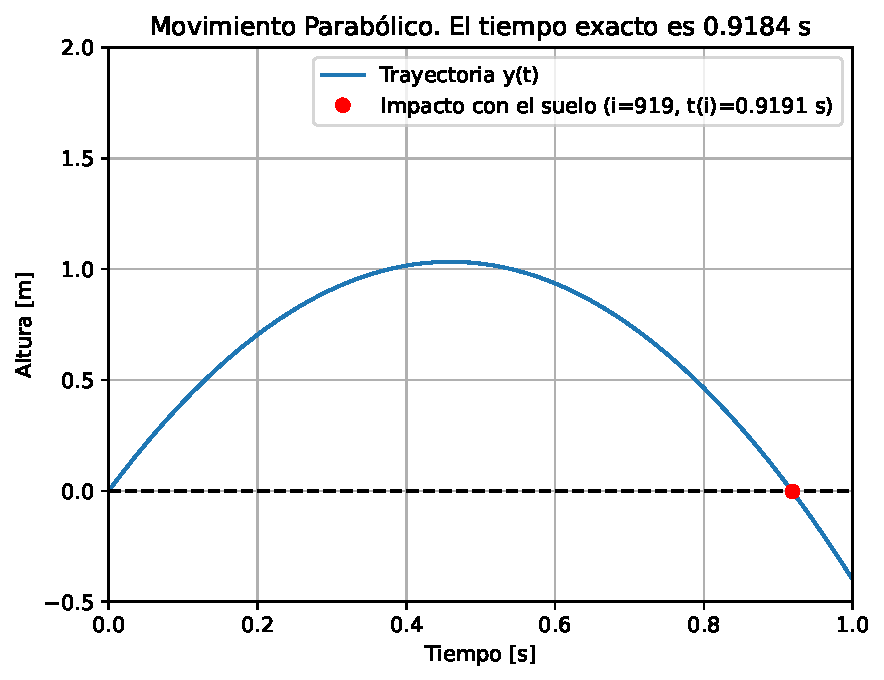
\includegraphics[width=0.7\textwidth]{parabolico.pdf}
    \caption{Gráfica de la altura $y$ en función del tiempo $t$ para $y_0 = 0$ m, $v_0 =4.5$ m/s.}
    \label{fig:yvst}
\end{figure}

\section*{\textcolor{red}{\textit{La libreria matplotlib}}}

Hasta el momento solo habíamos creado programas donde se visualizaban entradas y salidas como 
números o palabras. En Física, usualmente, dicen más los plots, como vimos en la sección anterior. 
En Python existen varias la librerías para graficar en Python, acá usaremos \textit{matplotlib}.
%
\begin{lstlisting}[language=Python, captionpos=t, title=\texttt{grafica\_simple.py}]
""" Uso básico de matplotlib"""
import matplotlib.pyplot as plt # cargamos la librería

#construimos listas
x = [0., 0.5, 1., 1.5, 2., 2.5, 3] 
t = [1., 1., 2., 3., 5., 8., 13.]

plt.plot(x,t)
plt.show()
\end{lstlisting}
%
En el código anterior (el más simple que podemo construir para graficar),
representamos un conjunto discreto de datos en el plano cartesiano.\\
\lstinline|import matplotlib.pyplot as plt|: importa la librería y le asocia el alias \lstinline|plt|.
Luego, se construyen las listas de datos. Es importante que ambas listas tengan el mismo
número de elementos. \lstinline|plt.plot(x,y)|: recibe las coordenadas y, por defecto, traza segmentos de 
línea recta entre los puntos consecutivos.  \lstinline|plt.show()|: muestra el gráfico. 
Acá se muestra una versión mejorada:
\begin{lstlisting}[language=Python, captionpos=t, title=\texttt{grafica\_simple\_v2.py}]
""" Uso básico de matplotlib"""
import matplotlib.pyplot as plt # cargamos la librería

#construimos listas
x = [0., 0.5, 1., 1.5, 2., 2.5, 3] 
t = [1., 1., 2., 3., 5., 8., 13.]

plt.plot(x,t,'r.',ms='15')
plt.xlabel(r'$x\,[\mathrm{m}]$',size=15)
plt.ylabel(r'$t\,[\mathrm{s}]$', size=15)

plt.savefig('grafica_simple_v2.pdf', bbox_inches='tight')
plt.show()
\end{lstlisting}
%
La salida se muestra en la figura \autoref{fig:grafica_simple_v2}
\begin{figure}[htbp]
    \centering
    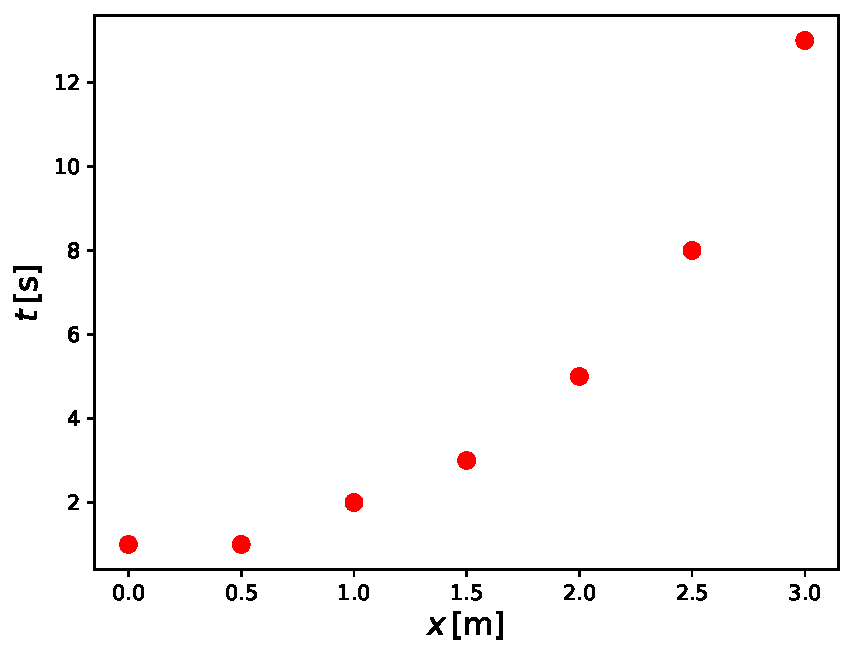
\includegraphics[width=0.7\textwidth]{grafica_simple_v2.pdf}
    \caption{Gráfica de la posición $x$ en función del tiempo $t$.}
    \label{fig:grafica_simple_v2}
\end{figure}
 
A continuación se detalla la sintaxis empleada en el código:

\begin{itemize}
    \item \texttt{plt.plot(x, t, 'r.', ms='15')}: Grafica la variable $x$ en el eje horizontal y $t$ en el eje vertical.
    \begin{itemize}
        \item \texttt{'r.'}: Define el estilo visual. La \texttt{'r'} asigna el color rojo (\textit{red}) y el punto \texttt{'.'} indica que los datos se representarán como puntos individuales sin líneas de interconexión.
        \item \texttt{ms='15'}: Ajusta el tamaño del marcador (\textit{marker size}) a $15$ puntos para facilitar su visualización.
    \end{itemize}
    
    \item \texttt{plt.xlabel(r'\$x\textbackslash,[\textbackslash{}mathrm\{m\}]\$', size=15)} y \\
    \texttt{plt.ylabel(r'\$t\textbackslash,[\textbackslash{}mathrm\{s\}]\$', size=15)}: Definen las etiquetas para los ejes horizontal y vertical, respectivamente.
    \begin{itemize}
        \item El prefijo \texttt{r} indica una cadena en formato ejecutable directo (\textit{raw string}), lo que evita que Python interprete caracteres de escape como \texttt{\textbackslash}.
        \item El entorno entre signos de pesos \texttt{\$...\$} invoca el motor interno de \LaTeX{} en Matplotlib.
        \item El comando \texttt{\textbackslash,} añade un espacio fino de separación entre la variable y las unidades.
        \item El comando \texttt{\textbackslash{}mathrm\{...\}} fuerza a que las unidades ($\mathrm{m}$ y $\mathrm{s}$) se desplieguen en texto romano (recto) y no en cursiva matemática, cumpliendo con la norma internacional de notación científica.
        \item \texttt{size=15}: Define un tamaño de fuente de $15$\,pt para las etiquetas.
    \end{itemize}

    \item \texttt{plt.savefig('grafica\_simple\_v2.pdf', bbox\_inches='tight')}: Exporta y guarda la figura generada en el disco duro.
    \begin{itemize}
        \item \texttt{'grafica\_simple\_v2.pdf'}: Nombre y formato de salida del archivo. Al usar la extensión \texttt{.pdf}, la gráfica se guarda en formato vectorial, lo que garantiza que no perderá calidad ni se pixelará al escalarla dentro de un documento impreso o un artículo en \LaTeX.
        \item \texttt{bbox\_inches='tight'}: Ajusta la caja delimitadora (\textit{bounding box}) de la figura de forma ajustada. Elimina los espacios en blanco innecesarios alrededor de la gráfica y evita que las etiquetas de los ejes (\texttt{xlabel} y \texttt{ylabel}) o la leyenda queden recortadas al exportar.
    \end{itemize}
    
    \item \texttt{plt.show()}: Despliega la ventana gráfica interactiva o renderiza la figura en el cuaderno de trabajo.
\end{itemize}

Para terminar, vamos a graficas un par de funciones conocidas. La salida se muestra en la figura \autoref{fig:funciones_simples}.
Para profundizar más en esta libreía, puede visitar la página oficial de \textit{matplotlib}
o mirar algunos ejemplos dando clic en este \href{https://matplotlib.org/stable/gallery/index.html}{enlace} y en este otro 
\href{https://matplotlib.org/stable/users/index.html}{enlace}.

\begin{lstlisting}[captionpos=t, title=\texttt{grafica\_funciones\_simples.py}]
""" Uso básico de matplotlib para graficar funciones simples"""
import matplotlib.pyplot as plt # cargamos la librería 
import numpy as np #cargamos numpy

#-----------
# figfura 1
#----------

teta = np.linspace(-2*np.pi, 2*np.pi, 100) # crea linspace
sint = np.sin(teta) # calcula el seno
cost = np.cos(teta) # calcula el coseno

plt.figure(1)
plt.plot(teta,sint,'r-',label= r'$\sin(\theta)$')
plt.plot(teta,cost,'b--',label= r'$\cos(\theta)$')
plt.xlabel(r'$\theta$', size=15)
plt.legend(loc='upper right')
plt.xlim(-2*np.pi, 2*np.pi)
plt.ylim(-1,1)
plt.savefig('senocoseno.pdf', bbox_inches='tight')

#----------
# figura 2
#-----------

x = np.linspace(0,100, 100)
logx = np.log(x) # note el error al calular el log0
sqrtx = np.sqrt(x)

plt.figure(2)
plt.plot(x,logx,'r-.',lw = '5', label= r'$\ln(x)$')
plt.plot(x,sqrtx,'b-',lw ='3.',label= r'$\sqrt{x}$')
plt.xlabel(r'$x$', size=15)
plt.legend(loc='upper left')
plt.xlim(0, 100)
plt.savefig('log10sqrt.pdf', bbox_inches='tight')

plt.show()
\end{lstlisting}

\begin{figure}[htbp]
    \centering
    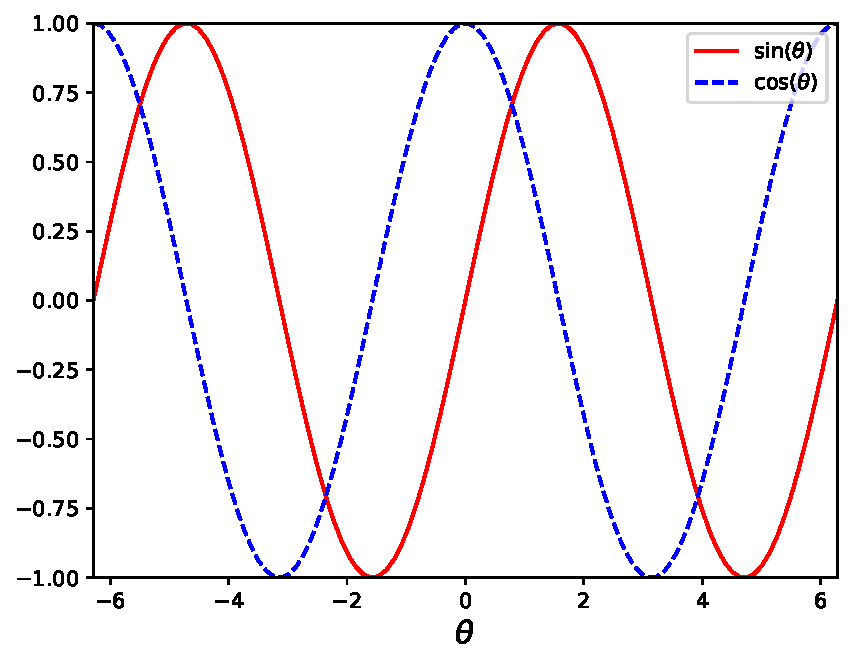
\includegraphics[width=0.48\textwidth]{senocoseno.pdf}
    \hfill
    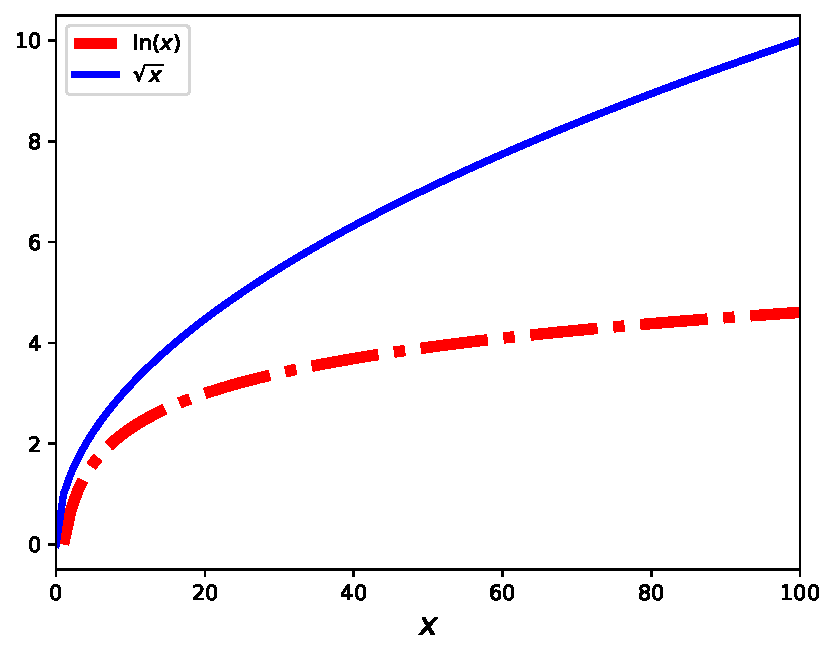
\includegraphics[width=0.48\textwidth]{log10sqrt.pdf}
    \caption{Gráficas de funciones simples usando Matplotlib.}
    \label{fig:funciones_simples}
\end{figure}

\begin{problemas}[]
\begin{enumerate}[leftmargin=*]

\item En física de la materia condensada, la \textit{constante de Madelung} da el potencial eléctrico total experimentado por un 
átomo en un sólido. Depende de las cargas de los otros átomos cercanos y de sus posiciones. Considere, por ejemplo, el cloruro de 
sodio sólido (la sal de mesa). El cristal de cloruro de sodio tiene sus átomos dispuestos en una red cúbica, 
pero alternando átomos de sodio y cloro; los de sodio tienen una sola carga positiva $+e$ y los de cloro una sola carga negativa $-e$, 
donde $e$ es la carga del electrón. Si etiquetamos cada posición de la red mediante tres coordenadas enteras $(i, j, k)$, 
los átomos de sodio se ubican en las posiciones donde $i + j + k$ es par, y los átomos de cloro en las posiciones 
donde $i + j + k$ es impar.

Considere un átomo de sodio en el origen, $i = j = k = 0$, y calculemos la constante de Madelung. 
Si la separación entre átomos en la red es $a$, entonces la distancia desde el origen hasta el átomo en la posición $(i, j, k)$ es:
\[
\sqrt{(ia)^2 + (ja)^2 + (ka)^2} = a \sqrt{i^2 + j^2 + k^2},
\]
y el potencial en el origen creado por dicho átomo es:
\[
V(i, j, k) = \pm \frac{e}{4\pi\epsilon_0 a \sqrt{i^2 + j^2 + k^2}},
\]
donde $\epsilon_0$ es la permitividad del vacío y el signo de la expresión depende de si $i + j + k$ es par o impar. 
El potencial total experimentado por el átomo de sodio es entonces la suma de esta cantidad sobre todos los demás átomos. 
Asumamos una caja cúbica alrededor del sodio en el origen, con $L$ átomos en todas las direcciones. Entonces:
\[
V_{\text{total}} = \sum_{\substack{i, j, k = -L \\ \text{no } i=j=k=0}}^{L} V(i, j, k) = \frac{e}{4\pi\epsilon_0 a} M,
\]
donde $M$ es la constante de Madelung. 

Escriba un programa para calcular e imprimir la constante de Madelung para el cloruro de sodio. 
Utilice un valor de $L$ tan grande como sea posible, asegurándose de que su programa se ejecute en un tiempo razonable (por ejemplo, 
en un minuto o menos).

\item En física nuclear, la \textit{fórmula semiempírica de masa} permite calcular la energía de ligadura nuclear aproximada $B$ 
de un núcleo atómico con número atómico $Z$ y número de masa $A$:
\[
B = a_1 A - a_2 A^{2/3} - a_3 \frac{Z^2}{A^{1/3}} - a_4 \frac{(A - 2Z)^2}{A} + \frac{a_5}{A^{1/2}},
\]
donde, en unidades de millones de electronvoltios ($\text{MeV}$), las constantes son $a_1 = 15.8$, 
$a_2 = 18.3$, $a_3 = 0.714$, $a_4 = 23.2$, y:
\[
a_5 = \begin{cases} 
0 & \text{si } A \text{ es impar,} \\ 
12.0 & \text{si } A \text{ y } Z \text{ son ambos pares,} \\ 
-12.0 & \text{si } A \text{ es par y } Z \text{ es impar.} 
\end{cases}
\]

\begin{enumerate}[label=\alph*)]
    \item Escriba un programa que tome como entrada los valores de $A$ y $Z$, e imprima la energía de ligadura para el 
    átomo correspondiente. Use su programa para encontrar la energía de ligadura de un átomo con $A = 58$ y $Z = 28$. 
    (\textit{Sugerencia: La respuesta correcta está alrededor de $500\text{ MeV}$}).
    
    \item Modifique su programa para que imprima no la energía de ligadura total $B$, sino la energía de ligadura por nucleón, 
    la cual es $B/A$.
    
    \item Ahora modifique su programa de modo que tome como entrada únicamente el valor del número atómico $Z$ y luego 
    recorra todos los valores de $A$ desde $A = Z$ hasta $A = 3Z$, para encontrar el que tenga la mayor energía de ligadura por 
    nucleón. Este es el núcleo más estable para el número atómico dado. Haga que su programa imprima el valor de $A$ para este 
    núcleo más estable y el valor de su energía de ligadura por nucleón.
    
    \item Modifique nuevamente su programa para que, en lugar de tomar $Z$ como entrada, recorra todos los valores de $Z$ 
    desde $1$ hasta $100$ e imprima el valor más estable de $A$ para cada uno. ¿Para qué valor de $Z$ ocurre la máxima 
    energía de ligadura por nucleón? (\textit{La respuesta real en la naturaleza es $Z = 28$, correspondiente al níquel}).
\end{enumerate}

\item Un proyectil se dispara desde el origen $(0,0)$ con una velocidad inicial $v_0 = 35.0\text{ m/s}$ y un ángulo de tiro $\theta = 42.0^\circ$.
    \begin{enumerate}[label=\alph*)]
        \item Calcule analíticamente el tiempo total de vuelo $T_{\text{vuelo}} = \frac{2 v_0 \sin\theta}{g}$ considerando $g = 9.81\text{ m/s}^2$.
        \item Genere un vector de tiempo continuo $t \in [0, T_{\text{vuelo}}]$ con $200$ puntos usando \texttt{numpy.linspace}.
        \item Escriba las ecuaciones vectorizadas para las posiciones $x(t) = v_0 \cos\theta \cdot t$ e $y(t) = v_0 \sin\theta \cdot t - \frac{1}{2}g t^2$.
        \item Grafique la trayectoria $y$ vs. $x$. Incluya en el título de la figura el tiempo de vuelo formateado a $4$ cifras decimales usando un \textit{f-string}.
    \end{enumerate}

    \item Considere la superposición de dos ondas armónicas con frecuencias ligeramente distintas $f_1 = 10\text{ Hz}$ y $f_2 = 12\text{ Hz}$ y la misma amplitud $A = 1.0$:
    $$y_1(t) = A \cos(2\pi f_1 t), \quad y_2(t) = A \cos(2\pi f_2 t)$$
    
    \begin{enumerate}[label=\alph*)]
        \item Construya un arreglo de tiempo $t \in [0, 2.0]$ segundos con $1000$ puntos.
        \item Evalúe $y_1(t)$ e $y_2(t)$, y obtenga la onda resultante por superposición $y_{\text{total}}(t) = y_1(t) + y_2(t)$.
        \item Consulte la función \lstinline|subplot| de 
        \textit{matplotlib} y genere una figura con dos subplots 
        verticales (\lstinline|plt.subplots(2, 1)|): el superior mostrando las 
        ondas individuales $y_1$ e $y_2$, y el inferior mostrando la onda de 
        resultante junto con su envolvente $A_{\text{env}}(t) = 2A \cos(\pi(f_1 - f_2)t)$.
    \end{enumerate}

    \item Aunque la función \lstinline|plot| está diseñada principalmente para graficar curvas estándar en coordenadas $xy$, también se puede adaptar para otro tipo de representaciones gráficas.

\begin{enumerate}[label=\alph*)]
    \item Realice un gráfico de la llamada \textit{curva deltoide}, la cual está definida paramétricamente por las ecuaciones:
    \[
    x = 2\cos\theta + \cos 2\theta, \quad y = 2\sin\theta - \sin 2\theta,
    \]
    donde $0 \le \theta < 2\pi$. Tome un conjunto de valores de $\theta$ entre $0$ y $2\pi$, calcule $x$ e $y$ para cada valor a partir de las ecuaciones anteriores y luego grafique $y$ en función de $x$.

    \item Llevando este enfoque un paso más allá, se puede realizar un gráfico en coordenadas polares $r = f(\theta)$ para alguna función $f$, calculando $r$ para un rango de valores de $\theta$ y luego convirtiendo $r$ y $\theta$ a coordenadas cartesianas mediante las ecuaciones estándar:
    \[
    x = r \cos\theta, \quad y = r \sin\theta.
    \]
    Utilice este método para graficar la \textit{espiral de Galileo} $r = \theta^2$ en el rango $0 \le \theta \le 10\pi$.

    \item Utilizando el mismo método, realice un gráfico en coordenadas polares de la \textit{"función de Fey"}:
    \[
    r = e^{\cos\theta} - 2\cos 4\theta + \sin^5\left(\frac{\theta}{12}\right)
    \]
    en el rango $0 \le \theta \le 24\pi$.
\end{enumerate}
\end{enumerate}
\end{problemas}

\label{LastPage}
\end{document}

